\documentclass[12pt]{article}

\usepackage{biblatex}
\addbibresource{bibliography.bib}

\usepackage{multicol}

\usepackage{amsfonts}
\usepackage{amsmath}

\usepackage{xcolor}
\usepackage{listings}

\usepackage{graphicx}
\graphicspath{ {./images/} }

\definecolor{mGreen}{rgb}{0,0.6,0}
\definecolor{mGray}{rgb}{0.5,0.5,0.5}
\definecolor{mPurple}{rgb}{0.58,0,0.82}
\definecolor{backgroundColour}{rgb}{0.95,0.95,0.92}

\lstdefinestyle{CStyle}{
	backgroundcolor=\color{backgroundColour},   
	commentstyle=\color{mGreen},
	keywordstyle=\color{magenta},
	numberstyle=\tiny\color{mGray},
	stringstyle=\color{mPurple},
	basicstyle=\footnotesize,
	breakatwhitespace=false,         
	breaklines=true,                 
	captionpos=b,                    
	keepspaces=true,                 
	numbers=left,                    
	numbersep=5pt,                  
	showspaces=false,                
	showstringspaces=false,
	showtabs=false,                  
	tabsize=2,
	language=C
}

\title{Reachability problems for counter automata}
\author{Lars Van Roy\\
\textit{dept. of Mathematics and Computer Science} \\
\textit{University of Antwerp}\\
lars.vanroy@student.uantwerpen.be}
\date{\today}

\begin{document}
\maketitle{}

\begin{abstract}
\noindent
Reachability is a known problem that can heavily affect the efficiency of code. It has been proven that reachability is decidable for one counter timed automata and to exploit this, we will create a program which will convert c code into such automata. In case the code conforms to the restrictions, enforced by the need of it being a one counter automata, a reachability test can be performed, but the latter will not be part of this research.
\end{abstract}

\section{Introduction}
A well known problem in writing code is the reachability of specific lines in set written code. It is often impossible to properly determine whether or not a line of code guarded by a condition statement is going to be reachable in any possible execution of the code. Unreachable code, due to unsatisfiable conditions, is an obvious issue for time restrained environments such as embedded computer systems. In order to upgrade the efficiency of code that is affected by time constraints, or code in general, a proper reachability analysis would be of great use. \newpage

In order to analyze code reachability, we will make use of a property proven by Daniel Bundala and Joal Ouaknine \cite{danialandjoel}, in which they state that reachability is decidable for timed automata with a single parametric clock. Adding the restriction of only allowing a single parametric clock has a big effect on the types of code we can analyse, but is unavoidable, since there is no proof for two counter machines. Three counter machines and up have been proven to be undecidable.

In this paper we will give an overview of a program which will be able to convert c code to such an automaton. The program will go through the following iterations on the path to generating a counter automaton.

\begin{enumerate}
	\item convert c code into a parse tree, using antlr
	\item perform context free reductions on this parse tree
	\item perform context sensitive reductions on this parse tree
	\item validate the resulting parse tree, to be conforming to the code constraints
	\item generate the counter automaton
\end{enumerate}

The c code can at most contain one counter (and preferably exactly one, as zero counter programs are assumed to be trivial when considering reachability). Furthermore, the operations on the counter will be restricted, the counter can only be altered via assignments with parameters or constants, and the counter can only be compared using equality, inequality, strict less than, strict greater than, less than or equal, greater than or equal, and only to paremeters or constants. Furthermore, these parameters can never be altered throughout the duration of the code.

Other then the described code constraint, functions must also have a boolean return type, and integer parameter types (if any) to be converted into a counter automaton.

\section{One counter automata}
The automata used in this project are a specific subset of the generally defined automata. The general definition for an automaton A is given by the tuple (S, $s_0$, $\delta$, F, Op, $\lambda$) where
\begin{itemize}
	\item S is the set of states
	\item $s_0$ is the set of initial states
	\item $\delta$ is the set of edges
	\item F is the set of final states
	\item Op is the set of operations
	\item $\lambda$ is the mapping for every edge to an element of the set of operations
\end{itemize}

A class of automata derived from the general automaton is the class of timed automata. Before we can consider a definition for these automata, we need to introduce a few additional concepts as described Martin Fr\^anzle et al. \cite{informationprocessingletters} and Uli Fahrenberg \cite{higherdimensionaltimedautomata}.

Consider a set of clocks $\chi$, the corresponding set $\phi(\chi)=\{x_1,...,x_n\}$ of clock constraints is generated corresponding to the following grammar $\varphi ::= true | x<k | x = k | x>k | \varphi\land\varphi$. where $k \in \mathbb{N}$ and $x \in \chi$. Hence $\phi(\chi)$ is nothing but a set of constraints based on conjunctions of comparisons with clocks to integers.

A clock valuation is a mapping $v:\chi \rightarrow \mathbb{R}_{\geq 0}$ where $\mathbb{R}_{\geq 0}$ is the set of non-negative real numbers. We denote $\mathbb{R}^{\chi}_{\geq 0}$ as the set of all clock valuations. Furthermore we write $v \models \varphi$ to denote that $v \in \mathbb{R}^{\chi}_{\geq 0}$ satisfies the constraint $\varphi$. We denote by 0 the valuation such that 0(x) = 0 for all $x \in \chi$. Given $t \in \mathbb{R}^{\chi}_{\geq 0}$, we let v+t be the clock valuation such that (v+t)(x) = v(x) + t for all clocks $x \in \chi$. Given $\lambda \subseteq \chi$, let v[$\lambda \leftarrow 0$] be the clock valuation such that
\[
	v[\lambda \leftarrow 0](x) = 
	\begin{cases}
		0,& \text{if } x \in \lambda\\
		v(x),& \text{if } x \notin \lambda
	\end{cases}
\]
A timed automaton B is defined by a tuple B = $(Q, q^0, Q^f, I, E)$, where
\begin{itemize}
	\item $Q$ is a finite set of locations
	\item $q^0$ represents the initial location, $q^0 \in Q$
	\item $Q^f$ represents the set of accepting locations, $Q^f \subseteq Q$
	\item $I$ assigns invariants to states, $I: Q \rightarrow \phi(\chi)$
	\item $E$ is the set of guarded transitions, $E \subseteq Q$ x $\phi(\chi)$ x $\Sigma$ x $2^\chi$ x $Q$
\end{itemize}

A run in a timed automaton is a sequence $\pi$ of configurations $c_1c_2 ... c_k$ such that each configuration is a direct successor of the previous configuration or, in other words, $c_i \rightarrow c_{i+1}$. We call a run accepting \textsl{accepting} if for a run $c_1c_2...c_k$ it holds that $c_1$ is the initial state and $c_k$ is the final state.

A one-counter automaton is a tuple $\mathcal{A}$ = $(Q, q_0, \sigma, F)$ where
\begin{itemize}
	\item $Q$ is a finite set of states
	\item $q_0 \in Q$ is the initial state
	\item $F \subseteq Q$ is the set of accepting states
	\item $\sigma \subseteq Q $ x $ L $ x $ Q $ is the transition relation with L the set of instructions
\end{itemize}

A counter valuation v is an element of $\mathbb{N}$ and a configuration of $\mathcal{A}$ is a pair in Q x $\mathbb{N}$. The initial configuration is the pair ($q_i$, 0). 

Finally, we will consider the following set of allowed operations where P is the set of parameters, the $\wedge$ symbol will be used to represent an empty label.
\[
 op = \{+c, -c, +p, -p, \leq c, =c, \geq c, \leq p, =p, \geq p: c \in \mathbb{N}, p \in P\} \cup \{\wedge\}
\]

The automata we will consider will be one-counter automata. The set $Q$ will contain a state for each line of code. The initial state $q_0$ will be the state corresponding with the first line of code. For now the set of final states $F$ will be empty, but the intended definition of the final state is the line(s) of which the reachability will be checked. The transition relation will consist of elements of the form $(q_i, l, q_{i+1})$ where $q_i, q_{i+1} \in Q$ and $l \in op$. For each element it will hold that we can reach line $q_{i+1}$ from $q_i$. The l element or operation can either be blank, in which case there is a statement on line $q_i$ but it has no effect on the evaluation of our counter and will therefore be disregarded, or not blank. The operation will always be part of the \textit{op} set described earlier.

There are a few exception to the above described states, some segments will have additional nodes to avoid confusion. In a loop there can be a pre loop, which will signify the state after the initial \textit{for condition} is performed, a start node for the inner segment, an end node to the inner segment, a post loop node, that will signify the state after the post statement has been evaluated, and finally a \textit{post iteration node}, which will signify the end of the statements. Same holds for selection statements (eg. if statements) which will have a start node, a start of success node, which signifies the body of the if statement, a start of else node, which will signify possible if else or else statements, and an end of selection node. Other states can be added for statements that require multiple steps, like assignments etc. These will be further explained in the generator section.
\subsection{division example}
Consider the following code segment, this code snippet will attempt to determine whether or not a given integer a, is greater or equal compared to a given integer b. Throughout the paper, the different steps will be described which will ultimately yield the automaton displayed in figure \ref{fig:greater_or_equal}.

\begin{lstlisting}[style=CStyle]
bool is_greater_or_equal(int a, int b){
	if(a >= b){
		return true;
	}
	return false;
}
\end{lstlisting}

\begin{figure}[h]
	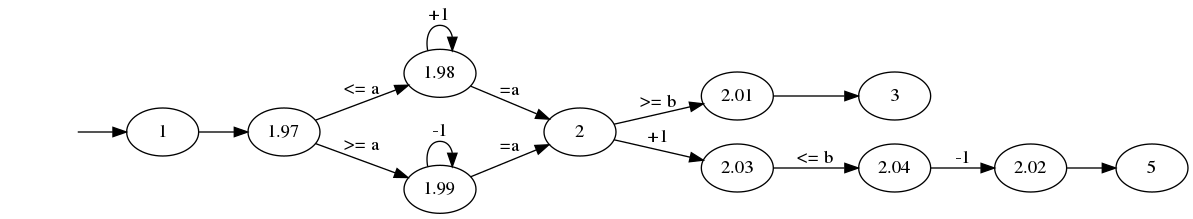
\includegraphics[width=\linewidth]{is_greater_or_equal_counter_automaton}
	\caption{A counter automaton corresponding with the is\_greater\_or\_equal function.}
	\label{fig:greater_or_equal}
\end{figure}

This example automaton $\mathcal{A}$ is defined by the tuple $(Q, q_0, \sigma, F)$, where
\begin{align*}
	Q &= \{1, 1.97, 1.98, 1.99, 2, 2.01, 2.02, 2.03, 2.04, 3, 5\} \\
	q_0 &= 1 \\
	\sigma &= \left\{ \begin{array}{l}
		(1, \wedge, 1.97), (1.97, \text{\textless =a}, 1.98), (1.98, \text{+1}, 1.98), (1.98, \text{=a}, 2), \\
		(1.97, \text{\textgreater =a}, 1.99), (1.99, \text{-1}, 1.99), (1.99, \text{=a}, 2), (2, \text{\textgreater =b}, 2.01),\\ (2.01, \wedge, 3), (2, \text{+1}, 2.03), (2.03, \text{\textless =b}, 2.04), (2.04, \text{-1}, 2.02),\\ (2.04, \wedge, 5)
	\end{array} \right\}\\
	F &= \emptyset
\end{align*}

\section{Program}
\subsection{Program overview}
The program that will perform the conversion from c code to a one counter automaton, will do this in five steps.

The first step, the initialization, will simply generate a parse tree, using the default c grammar, with the addition of the boolean type, and the removal of some gcc extensions.

The second step, the context-free abstract syntax tree generation, will generate an abstract syntax tree without any regard for neighboring nodes.

In the third step, the abstract syntax tree generated in the previous step will be simplified in a context-sensitive manner, which means that the program will now look at all neighboring nodes. All redundant nodes will be removed, so that only important nodes with unambiguous meaning remain.

The fourth step will be an analysis on whether or not the resulting abstract syntax tree conforms to all earlier specified requirements and, if this is the case, we will continue with the fifth step, which will be the generation of the counter automaton.

We will allow all counter operations that can directly be supported by the $op$ set described earlier. We will add assignment and inequality to this, as these can easily be represented as sequences of operations in the $op$ list. Along with these we will also need support for strict less than and greater than, which can also be implemented using the operations in the \textit{op} list. The full explanation on how this can be done, can be found in the generator section.

\subsection{Initialization}
The program will start of by running the generator antlr compilation unit on the given c code. In case there are any issues regarding simple compilation rules, the program will exit with an error, indicating the issues in the code. For the remainder of the execution, the code is assumed to be correct, and there will be no regard for potential issues within the code.

\subsection{Context-free abstract syntax tree generation}
Using the parse tree resulting from the antlr compilation, we will try to generate an abstract syntax tree that is as simple as possible without regarding any context. 

First of all, the code uses the notion of a node stack, this node stack will be used to store the nodes that are currently being evaluated.

The first loop will operate as a visitor, which will traverse the parse tree in a depth first manner. The first discovery of a node is done by calling the enter function corresponding to the type of node. As soon as all children of set node have been evaluated, the corresponding exit function will be called. 

However, the creation of nodes is not the same in all situations, in some cases, a specific kind of node will be created, and in other cases a specific kind of node will not be created, depending on the rule used for the current node (which we can determine from the context of the current node). In order to know whether or not we need to pop a node from the node stack, we will allow the code to look at the top node in the stack, and evaluate the type of set node. No other context related evaluations will be allowed.

\subsubsection{Context-free analysis assignmentExpression example}
To look at a concrete example, consider the following rule in the grammar:
\begin{align*}
	&assignmentExpression\\
	&\text{:}\indent \text{conditionalExpression}\\
	&|\indent \text{unaryExpression assignmentOperator assignmentExpression}\\
	&|\indent \text{Digitsequence}; \\
\end{align*}
The rule for conditionalExpression needs to be there, as there is a chain of expressions, and some expressions need to be higher in the order than others, therefore all expressions with a higher priority need to be evaluated before the lower priority expressions. This is done by adding a rule to a lower priority expression in each expression class. It is however undesirable for these nodes to be added. Without regard for context in other nodes, we can simply look at the current node to see whether or not the conditionalExpression line is used (which antlr generated context allows us to do).

Since there is a chance no new node was added within the enter function, we will also be required to evaluate the top of the stack, to see whether or not the top of the stack is a node we need to pop, the code will do the same check that was done in the enter function of the traversal.

\subsection{Context-sensitive abstract syntax tree reduction}
Now that all obviously redundant nodes have been eliminated, there is still the need for context sensitive reductions. We will attempt to implement constant propagation and substitution, in which we compute constant expressions, and replace variables with known value, by their actual value. Furthermore we will try to rephrase expressions by expressions with the same meaning, so that all expressions, if possible, are in an acceptable format for the counter automaton.

The context-sensitive reduction will also keep track of a lot of data about the variables in a symbol table. It will track whether or not variables are current initialized with a known value, values at certain points within the execution, it will track struct, union and enum definitions used for folding and so on. It will keep track of the kind of variables we have (eg. counters and parameters). All of this info will be used to enable the operations this cycle will perform, but will also be used in the validation loop.

The program will do this by traversing the abstract syntax tree resulting from the previous step, but will now specifically go through the children of relevant expressions (eg. assignment expressions, additive expressions, ...).

Important to note is that no folding/substitution will occur within loops, as these operations occur a variable number of times, and since there is no way of determining the exact number of times without evaluating the expression, this is considered too complex and often impossible, as counters may depend on parameters, which need to be chosen at evaluation time.


\subsubsection{Context-sensitive reduction example constant propagation}
Another example of a needed reduction, is constant propagation and folding. It is possible that a code segment would initially be rejected, due to use of unwanted variables, while in essence, these variables are nothing but variable representations of results of constant expressions. Consider the code snippet below. It would initially be rejected, because the counter variable is initialized with a variable that is neither a constant nor a parameter.
\newpage
\begin{lstlisting}[style=CStyle]
bool divide(int p, int n){
	int variable = 5;
	variable += 20;
	int counter = variable;
	while(counter > 0){
		counter -= n;
	}
	counter += 1;
	counter -= 1;
	if(counter == 0){
		return true;
	}
	return false;
}
\end{lstlisting}

However, due to constant propagation and folding, we can simplify the two statements on line 2 and line 3, so that they become.

\begin{lstlisting}[style=CStyle]
int variable = 25;
\end{lstlisting}

Now that the variable is just a constant, we can substitute this variable in the declaration of counter, so that we now have the following.
\begin{lstlisting}[style=CStyle]
int variable = 25;
int counter = 25;
\end{lstlisting}

The new code segment is acceptable, but we will not stop here, as the first line of the code is useless. It has no further benefit for the execution and will therefore be dropped. The final counter assignment will not be folded. Whenever a variable gets altered within a conditional scope, the variable is considered to be uncertain, and further folding based on earlier values will not be allowed. The final code segment is as described below, which is trivially accepted to be converted to a counter automaton.

\begin{lstlisting}[style=CStyle]
bool divide(int p, int n){
	int counter = 25;
	while(counter > 0){
		counter -= n;
	}
	counter += 1;
	counter -= 1;
	if(counter == 0){
		return true;
	}
	return false;
}
\end{lstlisting}

\subsubsection{Context-sensitive reduction example addition folding}
As described earlier, we do allow additions and subtractions of the form - v and + v, where $v \in P$ or $v \in \mathbb{N}$ with $P$ the set of parameters. Given that the formation described in figure \ref{fig:unfolded_addition} occurs in the automaton, we would technically not be allowed to accept this, as this is not directly in the specified format.

\begin{figure}[h]
	\centering
	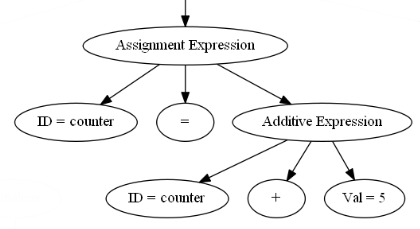
\includegraphics[width=0.8\linewidth]{unfolded_addition}
	\caption{An Assignment Expression with counter addition as value.}
	\label{fig:unfolded_addition}
\end{figure}

However, the context-sensitive reduction will be able to reduce the earlier specified example to the automaton in figure \ref{fig:folded_addition} This automaton will be acceptable, as this is a direct use of an allowed operation.

\begin{figure}[h]
	\centering
	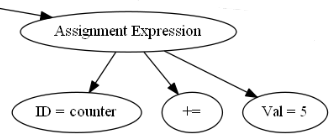
\includegraphics[width=0.6\linewidth]{folded_addition}
	\caption{An Assignment Expression with constant as value.}
	\label{fig:folded_addition}
\end{figure}
\newpage
\subsubsection{Nodes}
After the cleaning cycle has finished, there will only be a relatively small set of nodes remaining. Below a quick overview and their meaning within the syntax tree.

\begin{multicols}{2}
	\noindent
	\textbf{Compilation Unit} indicates the root of each Abstract Syntax Tree.\\
	\textbf{Function Definition} indicates the definition of a new function.\\
	\textbf{Function Specifier} indicates specifier of function.\\
	\textbf{Generic} head node for generic specification.\\
	\textbf{Generic Association} indicates a generic association.\\
	\textbf{Parameter Type List} head of the specification of all parameters of a function.\\
	\textbf{Parameter Declaration} head node of the declaration of a single parameter.\\
	\textbf{Compound Statement} indicates a scope defined by \{ \} brackets.\\
	\textbf{Type Specifier} indicates that the child(ren) of this node need to be regarded as being known type(s).\\
	\textbf{Type Name} indicates that the child(ren) of this node need to be regarded as being a type(s).\\
	\textbf{Type Def Name} indicates the definition of a type.\\
	\textbf{Declaration} indicates a declaration, this can contain multiple types and identifiers. In case of a function, the function name and parameter types plus identifiers will all belong to a single declarator node.\\
	\textbf{Init Declarator} defines a declaration of a variable with an initial value.\\
	\textbf{Direct Declarator} defines a declaration of a variable with a second variable.\\
	\textbf{Declarator} head node for the variable name part of the declaration.\\
	\textbf{Initializer} head node for the value part of the declaration.\\
	\textbf{Primary Expression} defines the most basic expression, eg. brackets, identifiers, constants, ... .\\
	\textbf{Postfix Expression} defines a postfix expression.\\
	\textbf{Unary Expression} defines a unary expression.\\
	\textbf{Cast Expression} defines a cast expression.\\
	\textbf{Multiplicative Expression} defines a multiplicative expression.\\
	\textbf{Additive Expression} defines an additive expression.\\
	\textbf{Shift Expression} defines a shift expression.\\
	\textbf{Relational Expression} defines a relational expression.\\
	\textbf{Equality Expression} defines an equality expression.\\
	\textbf{Bitwise And Expression} defines a bitwise and expression.\\
	\textbf{Bitwise Xor Expression} defines a bitwise exclusive or expression.\\
	\textbf{Bitwise Or Expression} defines a bitwise inclusive or expression.\\
	\textbf{Logical And Expression} defines a logical and expression.\\
	\textbf{Logical Or Expression} defines a logical or expression.\\
	\textbf{Conditional Expression} defines a conditional expression.\\
	\textbf{Assignment Expression} defines an assignment expression.\\
	\textbf{Expression} head node in case of multiple expressions.\\
	\textbf{For Declaration} head node for the first clause of a for loop.\\
	\textbf{For Expression} head node for a clause of a for loop.\\
	\textbf{For Condition} head node for the condition part of the second clause of a for loop.\\
	\textbf{Iteration Statement} defines an iteration statement (for, while, do while).\\
	\textbf{Jump Statement} defines a jump statement.\\
	\textbf{return} indicates return statement.\\
	\textbf{Labeled Statement} indicates a labeled statement.\\
	\textbf{Struct or Union Specifier} indicates the specification of a struct or union.\\
	\textbf{Enum Specifier} indicates the specification of an enumerator.\\
	\textbf{Struct Declaration} head node for a struct declaration.\\
	\textbf{Struct Declarator} head node for a struct declarator.\\
	\textbf{Static Assert Declaration} defines static assertion.\\
	\textbf{Enumerator} specifies variables part of an enumerator.\\
	\textbf{Size} head for array size.\\
	\textbf{Default} defines the default option for switch statement.\\
	\textbf{Alignment Specifier} defines an alignment restriction to an identifier.\\
	\textbf{Atomic Type Specifier} defines an atomic type.\\
	\textbf{Arguments} head node for arguments part of a function call.\\
	\textbf{sizeof} defines sizeof operation.\\
	\textbf{\_Alignof} defines \_alignof operation.\\
	\textbf{Val = $<$value$>$} defines a constant. \\
	\textbf{ID = $<$id$>$} defines a variable name.
\end{multicols}

\subsection{Abstract syntax tree validation}
The fourth loop will iterate over the abstract syntax tree resulting from the previous step, and while doing so, it will evaluate the nodes that occur and the context in which they occur.

The majority of the node evaluation is represented in a list of unsupported nodes. Most of these nodes are head nodes for certain kinds of expressions which will never be supported.

\begin{align*}
	unsupported = \left\{ \begin{array}{l}
		Multiplication\ Expression, sizeof, \_Alignof, \\
		\&, *, -, +, ., ->, !, ~, Cast\ Expression, \\
		Shift\ Expression, Bitwise\ And\ Expression, \\
		Bitwise\ Or\ Expression, Bitwise\ Xor\ Expression, \\
		*=, /=, \%=, <<=, >>=, \&=, ^=, |=, \\
		Logical\ And\ Expression, Logical\ Or\ Expression, \\
		Additive\ Expression
	\end{array} \right\}
\end{align*}

Whenever such a node occurs, the current situation will be inspected. We can either be assigning to a counter, or in a restricted conditional expression. The correct error will be chosen if either of the two situations is relative.

Furthermore, all variable usage will be tracked. We will allow multiple counters to exist, as long as we can substitute one general counter without having any conflicts, in other words, there can't be any overlap between counter usages. This is simply tracked by tracking the nodes in which the counter variables occur, with the exception of when they occur within conditional scopes. If this is the case, their first usage is set to the first line of the scope, so that overlap does occur when a different counter is used for the condition of the scope. 

Finally, the initial value will be tracked. In case there is a declaration with an initial value, this value will be chosen, otherwise it will be set to 0, which is the default integer value in C. This initial value allows us to skip over declarations in the generator. We can simply set the counter value to the initial value of the used counter at that point in time, just before its first usage.

Another aspect that will be tested, is the function definition. A function needs to have a boolean return type, and can only have integer parameters. If this not the case, an error status will be added.

These conditions will all be tracked separately for each function. Whenever the status list is empty at the end of the evaluation, we assume that no issues occurred, and we say that the function satisfies the requirements, if there are any issues, no counter automaton will be generated, and the errors will be printed to the terminal.

Important to note is that there is no regard for global statements. These are considered to be variable and undetermined. It could be that they can perfectly be used as counters, and that they will never be altered by other functions, but it is impossible to determine this efficiently. Therefore, a counter must be declared within the function scope.

\subsubsection{validation example}
When we go back to the earlier mentioned segment of code. We obtain the automaton displayed in figure \ref{fig:divide_cleaned}.

\begin{lstlisting}[style=CStyle]
bool divide(int p, int n){
	int counter = p;
	
	while(counter > 0){
		counter -= n;
	}
	
	if(counter == 0){
		return true;
	}
	return false;
}
\end{lstlisting}

\begin{figure}[h]
	\centering
	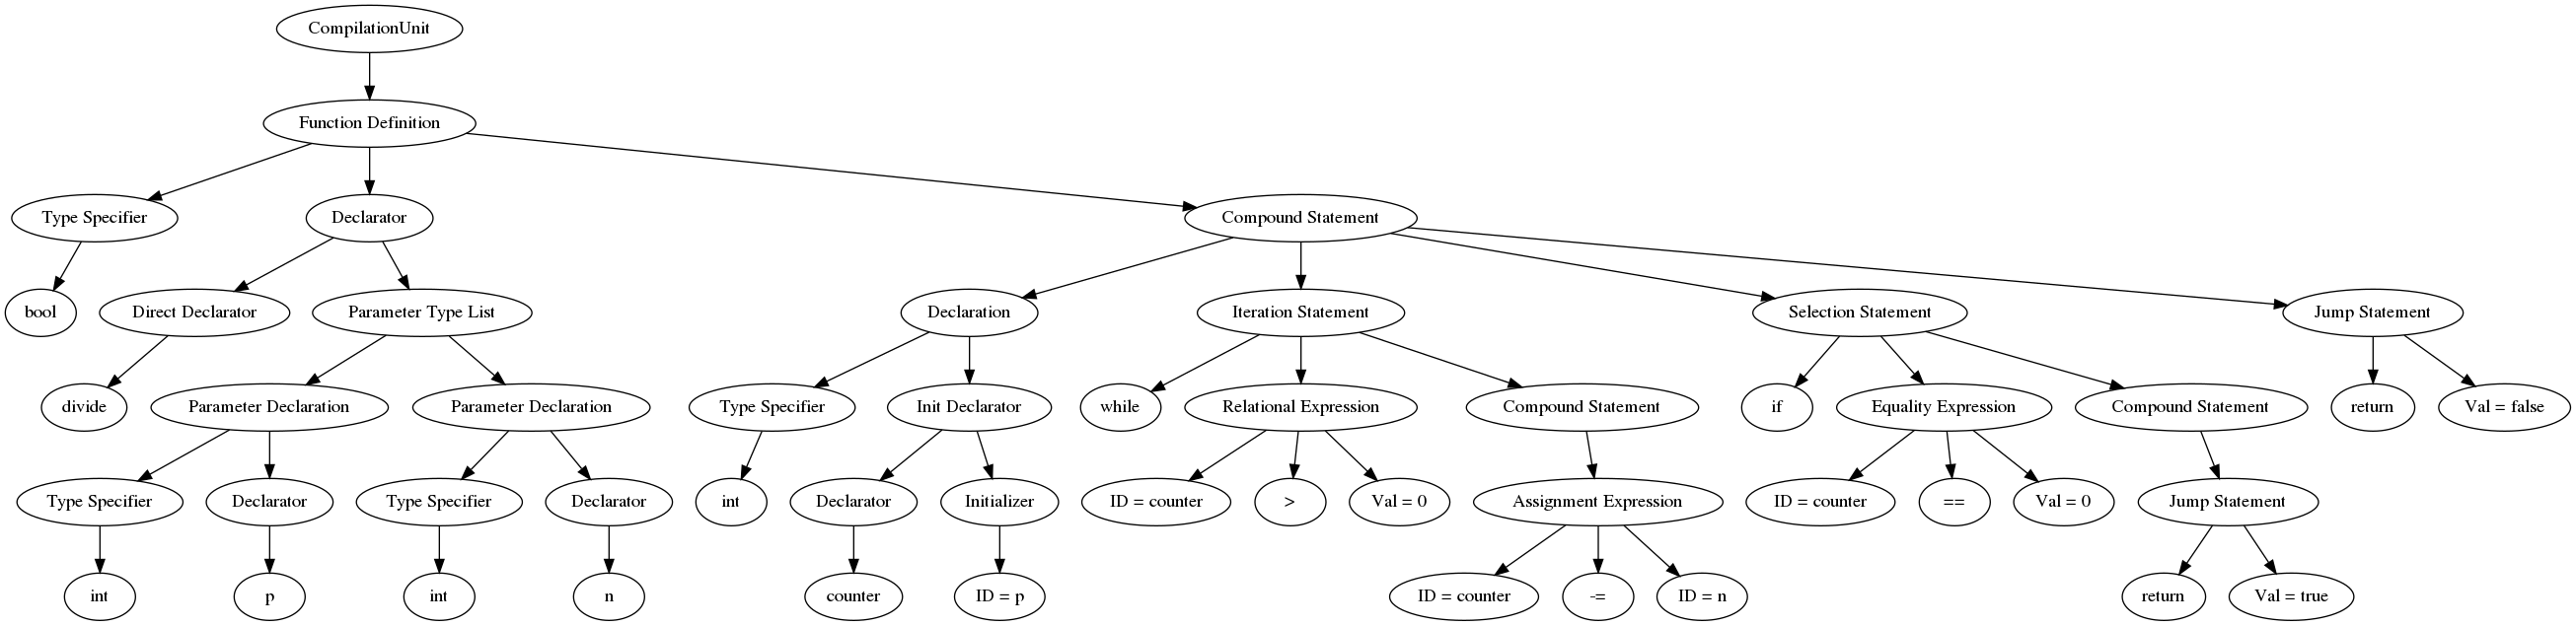
\includegraphics[width=\linewidth]{divide_cleaned}
	\caption{The cleaned Abstract Syntax Tree of the divide function.}
	\label{fig:divide_cleaned}
\end{figure}

We can immediately see that the function conforms to the required function definition, as the return type is boolean, as can be seen from the leftmost node. The parameters are also of type int, which can be seen from the parameters defined underneath the 'Parameter Type List' node.

From the cleaner we know which variables are counters, and we can see that the first declaration is a counter, but we will skip the declaration, as we know the value which is stored in the initial value, the initialization will happen before the first operation on the counter occurs. 

Next thing we encounter is the Iteration statement, for which we will check the condition with the constrained conditional variable enabled. With this variable enabled, we can simply continue traversing the nodes, and in case there are any unsupported nodes, the corresponding error would automatically be generated. However, there will be no corresponding nodes, so we will leave the Relational Expression without any error statuses, and we will disable the constrained conditional variable. 

Next we will enter the compound statement, which symbolizes the inner scope of the iteration statement. We will encounter an Assignment Expression with a variable that we know is a counter, we will therefore enable the counter assignment variable, while traversing the children of this node. No invalid nodes will appear, and we will disable the counter assignment variable when leaving the Assignment Expression node. 

The selection statement will be evaluated in the exact same manner as the Iteration Statement was evaluated, and as the jump statement holds no special operations, we can conclude that this function is ok for counter automaton generation.

\subsection{Counter automaton generation}
The final section of the program will be the counter generation itself. In this loop, there will be no more regards to possible invalid statements. At this point we assume everything to be known, and we can therefore simplify things drastically. Recall that the following list is the collection of allowed labels for the counter automaton.
\[
op = \{+c, -c, +p, -p, \leq c, =c, \geq c, \leq p, =p, \geq p: c \in \mathbb{N}, p \in P\} \cup \{\wedge\}
\]
This allows us to just check the head nodes related to such expressions.

An important thing to remark, is that we are not interested in general properties of runs for these automata. We are interested in the possibility of reachability or in other words, the existence of one path that will take us to a given node. This assumption is later on used to justify certain compositions.

\subsubsection{Functions}
First of all, we need the notion of the Function Definition statements. The generator will generate a counter automaton for each function, and needs to know when these start.

\subsubsection{Assignments}
Other than Functions, we will also need to know when assignments to counters occur, so that we can add the proper transition labels. We only need to check whether or not we are assigning to a counter, if so, we read the operation used, and the variable that gets assigned, and the manner $\in \{=, +=, -=\}$ gets used. 

As mentioned earlier, assignments are not in the set of operations, but they can be represented using the operators displayed earlier, as can be seen in figure \ref{fig:counter_assignment}. This can be done by using a reset operation, where we first check whether or not the counter is smaller or equal to the desired value, if so, it is either already satisfied, in which case we can just carry on, or it is smaller than the desired value, for which we will add a self loop with $+1$ as a label, so that we will eventually reach the desired value. The same sequence of events occur in case the counter is larger or equal to the desired value, with the exception that we will use $-1$ as an in between operation.

\begin{figure}[h]
	\centering
	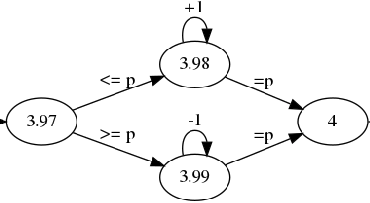
\includegraphics[width=0.48\linewidth]{counter_assignment}
	\caption{Assignment of a value p to a counter.}
	\label{fig:counter_assignment}
\end{figure}

The same thing can be done when the counter is larger or equal to the desired value, if so, it is either already satisfied, in which case we can just carry on, or it is larger than the desired value, at which point we will decrement the counter with a self loop of -1, until the condition is satisfied.

This can be done without adding additional weightings to transitions, due to the remark made earlier. We are not interested in properties for every single run, yes there are runs where the counter can loop infinitely, but there will also be a run where the counter gets to the correct value, after which it will continue onward.

\subsubsection{Loop statements}
We will also need the notion of selection statements. These will make use of a maximum of 5 nodes to enforce everything related to the loops. 

The first node will be the $start$ of the conditional statement, the second node is the pre node. This node symbolizes the state after the precondition of the for loop has been evaluated. 

Next we need a node to identify the $start\ of\ the\ inner\ segment$, which will be reached by a transition with the condition as a label. 

After this node the inner segment will follow, and it will be finalized with the $stop\ inner\ segment$ node, in case this one is needed. This stop node will symbolize the state after the post expression of the for loop has been evaluated, after this node, a transition will occur to the pre node, to reevaluate the loop condition.

Finally, one more node is needed, and this node will symbolize the \textit{end of the loop}. This node will always be the last node that gets generated, so that any nodes generated beyond this point will start from this point.

Consider the following segment of code.
\begin{lstlisting}[style=CStyle]
bool test(int a){
	int counter = 25;
	for(counter = 0; counter < 5; counter ++){
		continue;
	}
	counter = counter + 5;
	return true;
}
\end{lstlisting}

\begin{figure}[h]
	\centering
	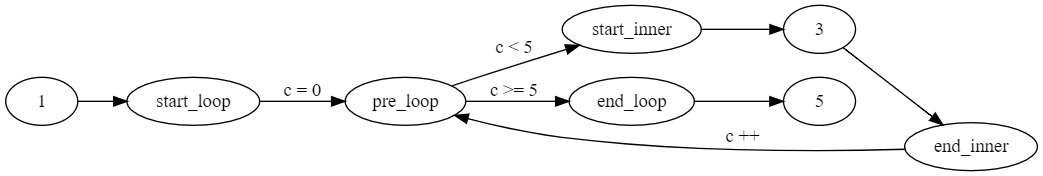
\includegraphics[width=\linewidth]{test_counter_automaton}
	\caption{Example of an Iteration Statement.}
	\label{fig:test_counter_automaton}
\end{figure}

This will result in the counter automaton seen in figure \ref{fig:test_counter_automaton}. The iteration start node will be node 3.01, the start of the inner segment will be node 3.06 and the end of this same segment 3.02.

The inner segment itself consists out of one single node, being node 4.

The end of the iteration is denoted by node 3.03, and the first node beyond the iteration statement, being node 6, will follow after this one.

\subsubsection{If statements}
Another important construct are the if statements. These statements will, just as the loop statements did, require additional nodes to be able to be modeled. If statements require a total of 4 nodes to be modeled.

First of all, we need a $start\ of\ the\ iteration\ statement$ node, from which the conditions will start.

We will need an $if\ node$ and an $else\ node$ which will both signify the start of the if and possible else segment.

After the inner segment, they will all end up at the $end\ of\ the\ iteration\ statement$ from which point they will continue with the next line of code.

Consider the test2 function, it contains an if statement, an else if statement and an else statement.
\begin{lstlisting}[style=CStyle]
bool test2(){
	int counter = 25;
	if(counter == 23){
		counter += 3;
	}
	else if(counter == 24){
		counter += 2;
	}
	else{
		counter += 1;
	}
	return true;
}
\end{lstlisting}

\begin{figure}[h]
	\centering
	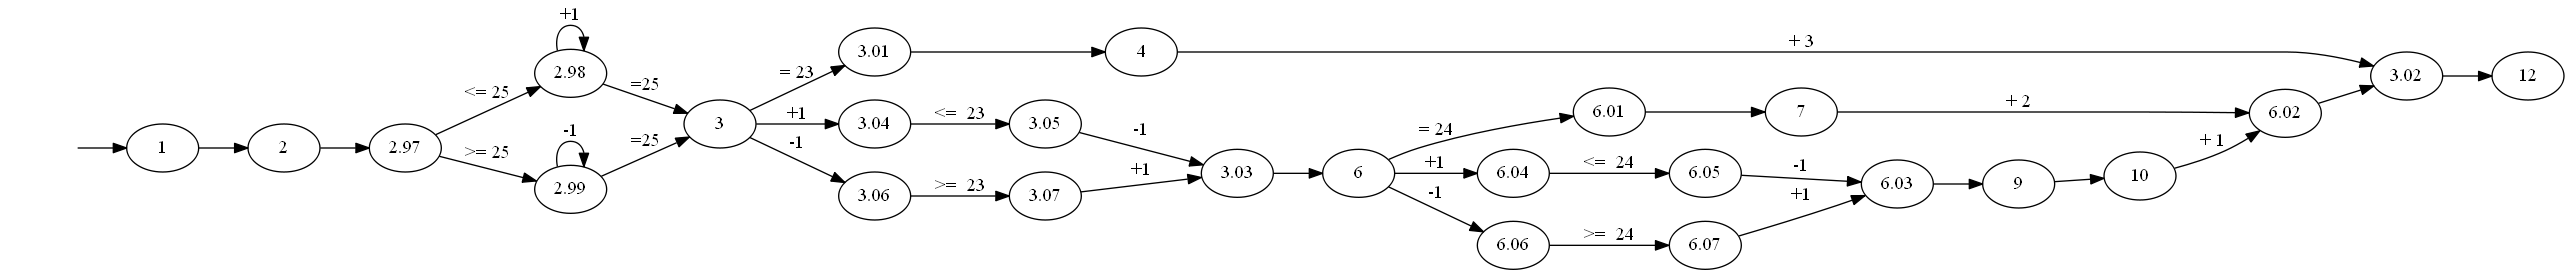
\includegraphics[width=\linewidth]{test2_counter_automaton}
	\caption{Example of Selection Statements.}
	\label{fig:test2_counter_automaton}
\end{figure}

The program will return a counter automaton as displayed in figure \ref{fig:test2_counter_automaton}. The iteration start node of the outer if will be node 3, the if node and else node of the same if will be 3.01 and 3.04 respectively. The end node of this if statement will be 3.02.

The else if will have 6 as a start node, 6.01 and 6.04 will function as if and else nodes respectively. Node 6.02 will signify the end of the else if statement.

Finally, the else statement will start at node 7, since this is no conditional statement, it will just behave as regular code.

\subsubsection{Inequality condtions}
Another statement we will need to support, are inequality conditions. If we want our conditional statements to be properly functioning, we will need to be able to generate opposing conditions, but the opposing condition of the equality condition, is the inequality condition, which we can not directly model using the given operations.

The following code segment makes use of an if statement which has an equality condition in it. This means that the edge going towards the else node, will have the opposing condition as a label.

\begin{lstlisting}[style=CStyle]
bool is_ten(int a){
	int counter = a;
	
	if(counter == 10){
		return true;
	}
	
	return false;
}
\end{lstlisting}

When looking at part of the resulting counter automaton in figure \ref{fig:inequality_expression}, we will notice the transitions going from the start of the if statement, being node 4, towards the end of the if statement, being node 4.02. There will not be an else node, as there is no else if or else statement.

\begin{figure}[h]
	\centering
	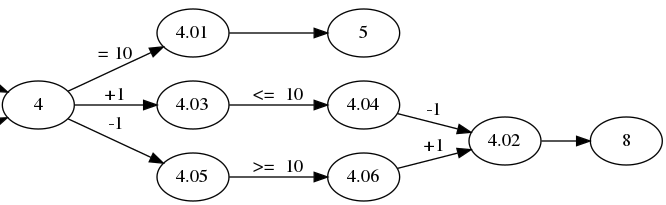
\includegraphics[width=\linewidth]{inequality_expression}
	\caption{Example of an inequality expression.}
	\label{fig:inequality_expression}
\end{figure}

The first transition chain starts with \textit{+1} followed by \textit{\textless =10}, followed by \textit{-1}, which results in the same expression as saying the original counter is strictly smaller than 10. The final \textit{-1} is there to reset the counter, so that the counter is back to what it originally was. 

The second transition chain start with \textit{-1}, followed by \textit{\textgreater =10}, followed by \textit{+1}. This chain states that the counter must be strictly greater than 10.

If either of these can be taken, we can state that the counter must be different to the compared value (in this case 10), as these both express a strict inequality. 

\subsubsection{less than and greater than}
The final additional expressions that will be added to the program described within his paper, are the less than and greater than expressions. These are needed to model the opposing conditions to greater than or equal and less than or equal respectively.

\begin{lstlisting}[style=CStyle]
bool is_ten(int a){
	int counter = 10;
	
	if(counter <= a){
		if(counter < a){
			return false;
		}
		return true;
	}
	
	return false;
}
\end{lstlisting}

The is\_ten code segment models both a less than or equal condition and a less than condition. This will mean that the first will need to be opposed with a strictly greater than condition, and the second one with a greater than or equal condition.

\begin{figure}[h]
	\centering
	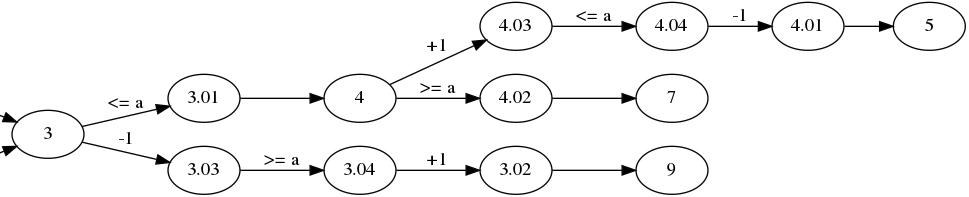
\includegraphics[width=\linewidth]{less_than_greater_than}
	\caption{Example of a less than expression and a greater than expression.}
	\label{fig:less_than_greater_than}
\end{figure}


Part of the counter automaton of the is\_ten function can be seen in figure \ref{fig:less_than_greater_than}. This automaton has 3 as the start of the outer if and it has 3.01 and 3.02 as respective if and end nodes. The inner if has 4 as the start node, 4.01 as the start of the if segment, and 4.02 as the end node.

The strict greater than condition, originating from node 3 and ending in node 3.02, consists of 3 different transitions. The first transition \textit{-1} and \textit{\textgreater =a}, test if the counter is strictly greater. The third transition \textit{+1} is there to make sure that the counter goes back to its original value.

The strict less than condition, originating from node 4 and ending in node 4.01, consists of \textit{+1} and \textit{\textless =a} as their first two conditions, which can only be satisfied in case the counter is strictly less than a. The final condition \textit{-1} is there to make sure the counter goes back to its original value.


\section{Conclusion}
In this paper we gave a brief description of a program capable of converting a small subset of the c language to counter automata, to be used in later evaluation of reachability. 

This subset consists of all functions who contain a maximum of one counter (and preferably exactly one, as reachability analysis without a single counter is considered trivial). The operations allowed on the counter are limited to addition and subtraction of parameters and constants, as well as assignment with parameters and constants. The conditional evaluations that are allowed are equality, inequality, strict less than, strict greater than, less than or equal and greater than or equal. All of these conditions must either be compared to constants or variables. Finally, variables can not be altered during the execution of the code and must remain constant.

The paper gives a description on all the steps the program goes through in order to achieve this counter automaton, as well as a brief insight in why things are the way they are.

The usability of this program without any further additions is very limited. The restrictions enforced on the c code make it fairly useless in more complex situations, where reachability analysis would be far more desired however, it is very effective in case the program is applicable. Big conditional statements or a large amount of conditional statements can make the reachability of certain sub segments hard, and with the addition of a reachability checker, they could definitely lead to improvements in coding.

\section{Future work}
In a future research, we will attempt to improve the given program, so that it will be more efficient, and most importantly, more useful. The program is too restrictive to be practically usable, and should therefore be expanded to support further c code.

Furthermore, in this same research we will add an expansion to the program, which will allow the evaluation of counter automata, so that actual reachability conclusions can be made.
\printbibliography
\end{document}